\documentclass[tikz,border=10pt]{standalone}
\usetikzlibrary{calc}

\begin{document}
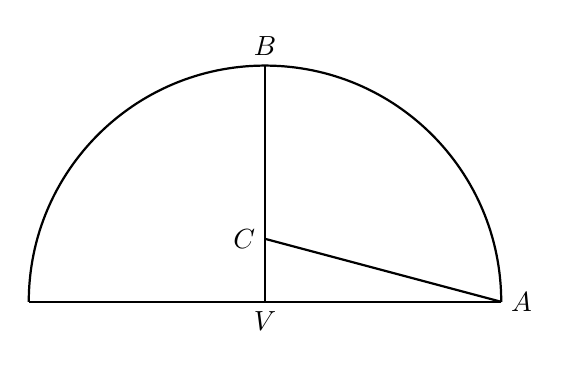
\begin{tikzpicture}
    % 定义参数
    \def\R{3} % 半圆半径
    
    % 定义坐标
    \coordinate (V) at (0,0);
    \coordinate (A) at (\R,0);
    \coordinate (B) at (0,\R);
    \coordinate (C) at (0,0.8); % 可调整C点在半径上的高度
    \coordinate (LeftEnd) at (-\R,0);

    % 绘制半圆弧
    \draw[thick] (LeftEnd) arc (180:0:\R);
    
    % 绘制底边线段
    \draw[thick] (LeftEnd) -- (A);
    
    % 绘制垂直线段 VB
    \draw[thick] (V) -- (B);
    
    % 绘制线段 CA
    \draw[thick] (C) -- (A);
    
    % 标注各点名称
    \node[below] at (V) {$V$};
    \node[right] at (A) {$A$};
    \node[above] at (B) {$B$};
    \node[left] at (C) {$C$};

\end{tikzpicture}
\end{document}